\documentclass[a4paper,14pt]{extreport} %размер бумаги устанавливаем А4, шрифт 12пунктов
\usepackage[T2A]{fontenc}
\usepackage[utf8]{inputenc}%включаем свою кодировку: koi8-r или utf8 в UNIX, cp1251 в 
\usepackage[english,russian]{babel}
\usepackage{amssymb,amsfonts,amsmath,mathtext,cite,enumerate,float}
\usepackage{hyperref}
\renewcommand{\rmdefault}{ftm}

\usepackage{geometry}
\geometry{left=3cm}
\geometry{right=1.5cm}
\geometry{top=2.0cm}
\geometry{bottom=2.0cm}

\renewcommand{\baselinestretch}{1.3}  % 1 интервал

\renewcommand{\thetable}{\arabic{section}.\arabic{table}}

%\renewcommand{\captionlabeldelim}{ \textendash}

\tolerance=10000

\newcommand{\D}{\mathrm{d}}
% Производные
\newcommand{\dsl}[2]{{\partial #1}/{\partial #2}}
\newcommand{\df}[1]{\cfrac{\partial}{\partial #1}}
\newcommand{\dff}[2]{\frac{\partial #1}{\partial #2}}
\newcommand{\dfs}[2]{\frac{\partial^2 #1}{\partial #2^2}}
\newcommand{\Df}[1]{\frac{d}{d #1}}
\newcommand{\Dff}[2]{\frac{d #1}{d #2}}
\newcommand{\Dfs}[2]{\frac{d^2 #1}{d #2^2}}
\newcommand{\cDf}[1]{\cfrac{d}{d #1}}
\newcommand{\cDff}[2]{\cfrac{d #1}{d #2}}
\newcommand{\cDfs}[2]{\cfrac{d^2 #1}{d #2^2}}
\newcommand{\dfn}[3]{\frac{\partial^#1 #2}{\partial^#1 #3}}
% Векторы
\renewcommand{\vec}[1]{\bm{#1}}
\newcommand{\ort}[1]{\bm{\mathrm{e}}_#1}
% Векторный анализ
\renewcommand{\div}{\mathrm{div}\,}
\newcommand{\rot}{\mathrm{rot}\,}
\newcommand{\grad}{\mathrm{grad}\,}
\newcommand{\laplas}[4]{\dfs{#1}{#2}+\dfs{#1}{#3}+\dfs{#1}{#4}}
\newcommand{\laplasxyz}[1]{\dfs{#1}{x}+\dfs{#1}{y}+\dfs{#1}{z}}
\newcommand{\rotc}[4]{\dff{#1}{#2} - \dff{#3}{#4}}
\newcommand{\rotcx}[3]{\dff{#1\vphantom{E}_#3}{#2} - \dff{#1\vphantom{E}_#2}{#3}}
% Функции
\renewcommand{\cosh}{\mathrm{ch}\,}
\renewcommand{\sinh}{\mathrm{sh}\,}
\renewcommand{\tanh}{\mathrm{th}\,}
\renewcommand{\Im}{\mathrm{Im}\,}
\renewcommand{\Re}{\mathrm{Re}\,}
\renewcommand{\det}[4]{#1 #4 - #2 #3}
\renewcommand{\matrix}[4]{\begin{pmatrix}#1 & #2 \\ #3 & #4\end{pmatrix}}
\newcommand{\matrixw}[5]{\begin{#5matrix}#1 & #2 \\ #3 & #4\end{#5matrix}} % #5 = b p s v V
\newcommand{\col}[2]{\begin{pmatrix}#1 & #2\end{pmatrix}}
\newcommand{\colw}[3]{\begin{#3matrix}#1 & #2 \end{#3matrix}} % #3 = b p s v V
\newcommand{\row}[2]{\begin{pmatrix}#1 \\ #2\end{pmatrix}}
\newcommand{\roww}[3]{\begin{#3matrix}#1 \\ #2 \end{#3matrix}} % #3 = b p s v V
\newcommand{\matrixrot}[2]{\begin{#2matrix} \ort{x} & \ort{y} & \ort{z} \\ \df{x} & \df{y} & \df{z} \\ #1_x & #1_y & #1_z \end{#2matrix}}
\newcommand{\matrixrotr}[4]{\begin{#4matrix} \ort{x} & \ort{y} & \ort{z} \\ \df{x} & \df{y} & \df{z} \\ #1 & #2 & #3 \end{#4matrix}}
\newcommand{\eps}{\varepsilon}
\renewcommand{\phi}{\varphi}

\newcommand{\shtr}{\mathop{\!\vphantom{E}'}}
\newcommand{\ind}[1]{\mathop{\!\vphantom{E}_{#1}}}
%\renewcommand{\theequation}{\arabic{section}.\arabic{equation}}

\usepackage[pdftex]{graphicx}
\usepackage{nccfloats}
% для цветного текста
\usepackage[usenames]{color}
%Рисунки в две колонки для окружения multicols
\usepackage{multicol}

\usepackage{mathrsfs} % буква для обозначения ЭДС
\newcommand{\EDS}{\ensuremath{\mathscr{E}}}
\newcommand{\Li}{\ensuremath{\mathscr{L}}}
\newcommand{\F}{\ensuremath{\mathscr{F}}}
\newcommand{\PP}{\mathop{\varPi\, }}
%жирные греческие буквы
\usepackage{bm}

%Настройка глав
\usepackage{titlesec}

\titleformat{\chapter}[display]
{\filcenter}
{}
{0em}
{\thechapter~}{}

\titleformat{\section}
{\normalsize}
{\thesection~}
{0em}{}

\titleformat{\subsection}
{\normalsize}
{\thesubsection~}
{0em}{}

\titleformat{\subsubsection}
{\normalsize}
{\thesubsubsection~}
{0em}{}

% Настройка вертикальных и горизонтальных отступов
\titlespacing*{\chapter}{0pt}{0pt}{0pt}
\titlespacing*{\section}{\parindent}{0pt}{0pt}
\titlespacing*{\subsection}{\parindent}{0pt}{0pt}

%Оглавление
\usepackage{tocloft}
\renewcommand{\cfttoctitlefont}{\hfill \MakeUppercase}
\renewcommand{\cftaftertoctitle}{\hfill}
\renewcommand{\cftbeforetoctitleskip}{0em}
\renewcommand{\cftchapfont}{\mdseries}
\renewcommand{\cftchappagefont}{\mdseries}
\renewcommand{\cftbeforechapskip}{0em}
\renewcommand{\cftdotsep}{1}
\renewcommand{\cftchapdotsep}{1}
\renewcommand{\cftchapleader}{\mdseries\cftdotfill{\cftchapdotsep}}
\setlength{\cftchapindent}{0pt}
\setlength{\cftsecindent}{0pt}
\setlength{\cftsubsecindent}{0pt}
\setlength{\cftsubsubsecindent}{0pt}
\setcounter{tocdepth}{3} % задать глубину оглавления — до subsection включительно

\usepackage{indentfirst} 

\usepackage[tableposition=top]{caption}
\usepackage{subcaption}
\DeclareCaptionLabelFormat{gostfigure}{Рисунок #2}
\DeclareCaptionLabelFormat{gosttable}{Таблица #2}
\DeclareCaptionLabelSeparator{gost}{~---~}
\captionsetup{labelsep=gost}
\captionsetup[figure]{labelformat=gostfigure}
\captionsetup[table]{labelformat=gosttable}
\renewcommand{\thesubfigure}{\asbuk{subfigure}}
\allowdisplaybreaks

\usepackage[square,numbers]{natbib}
\renewcommand{\bibsection}{\centering{\MakeUppercase{Список использованных источников}}}
\makeatletter
\renewcommand\@biblabel[1]{#1} % No brackets for the references
\renewenvironment{thebibliography}[1]
{	
	\bibsection
	\list{\@biblabel{\@arabic\c@enumiv}}%
	{\settowidth\labelwidth{\@biblabel{#1}}%
		\leftmargin0pt
		\setlength\itemindent{\dimexpr\labelwidth+1.25cm}% change using the inverse of the length used before
		\setlength{\parsep}{0pt}
		\@openbib@code
		\usecounter{enumiv}%
		\let\p@enumiv\@empty
		\renewcommand\theenumiv{\@arabic\c@enumiv}}%
	\sloppy
	\clubpenalty4000
	\@clubpenalty \clubpenalty
	\widowpenalty4000%
	\sfcode`\.\@m}
{\def\@noitemerr
	{\@latex@warning{Empty `thebibliography' environment}}%
	\endlist}
\renewcommand\newblock{\hskip .11em\@plus.33em\@minus.07em}
\makeatother

\parindent=1.25cm
\usepackage{enumitem}
\makeatletter
\AddEnumerateCounter{\asbuk}{\@asbuk}{м)}
\makeatother
\setlist{nosep,wide}

\newcommand{\ultext}[4]{
	\parbox[t]{#1}{
		\centering
		\underline{\hspace{#2}#3\hspace{#2}}\\
		\vspace{-3mm}
		{\footnotesize\hfill#4\hfill}
	}	
}

\newcommand{\uldate}[3]{
	<<#1>>~#2~#3~г.
}

\hyphenation{ВолгГТУ}
\begin{document}
\renewcommand{\contentsname}{Содержание}

\begin{titlepage}
	\begin{center}
		Государственное бюджетное образовательное учреждение высшего
		профессионального образования\\
		«Волгоградский государственный технический университет»\\
		\vspace{1em}
		Факультет электроники  и  вычислительной  техники\\
		\vspace{0.6em}
		Кафедра физики\\ 
	\end{center}
	\begin{flushright}
		УТВЕРЖДАЮ\\
		\vspace{0.6em}
		\parbox{7cm}{
		Научный руководитель профиля \\
		магистерского направления
		}\\
		\vspace{1em}
		\ultext{7cm}{1cm}{~~~~проф., д. ф.-м. н.~~~~}{}\\
		%\ultext{7cm}{3.5cm}{}{Учёная~степень{,}~учёное~звание}\\
		\vspace{1em}
		\ultext{6cm}{0.5cm}{~~~~~~~~~~~~~~~~~Шеин А. Г.}{Подпись~~~~~~~~~~~~~~~~~~~~~~}\\
		%\ultext{6cm}{3cm}{}{Подпись~~~~~Фамилия~и~инициалы}\\
		\uldate{\underline{~~}}{\underline{~~~~~~~~~}}{2014}
	\end{flushright}
	\vfil
	\begin{center}
		ОТЧЕТ\\
		О  НАУЧНО-ИССЛЕДОВАТЕЛЬСКОЙ РАБОТЕ\\
		\vspace{1em}
		Взаимодействие релятивистского электронного потока с электромагнитным\\
		полем замедляющих структур в приближении малой амплитуды сигнала\\
		(промежуточный, 1 семестр)
	\end{center}
	Студент \hfill Ф-1н Аликов Сергей Александрович \ultext{4cm}{2cm}{}{Подпись и дата}\\
	Научный руководитель магистерской диссертации \hfill
	\begin{flushright}
		\underline{к.~ф.-м.~н.,~доц.,~Ковтун~Д.~Г.}
	\end{flushright}
	\vfill
	\begin{center}
		Волгоград 2014
	\end{center}
\end{titlepage}

\setcounter{page}{2}

\begin{center}
	\MakeUppercase{Реферат}
\end{center}

Отчёт 25 с., 2 ч., 9 рис., 32 источника.

В работе сделан обзор литературы по методам расчёта электронных потоков, и работам, связанным с замедляющими структурами. Проведены расчёты потоков в структуре типа "гребёнка над плоскостью" с использованием выражений для магнитных полей структуры. Обнаружено сильное влияние магнитных полей структуры на форму электронных потоков. Также проведены расчёты потоков при условии, что на поток действует несколько гармоник поля структуры.
~\\

Ключевые слова: электронный поток, замедляющая структура, гребёнка, гребёнка над плоскостью, методы "частица-частица".

\newpage

\tableofcontents

\newpage

\addcontentsline{toc}{section}{Введение}

\begin{center}
	\MakeUppercase{Введение}
\end{center}

Применение устройств, принцип действия которых основан на использовании электронного потока, по-прежнему остаётся актуальным. В большинстве таких приборов используется взаимодействие электронного потока с электромагнитным полем замедляющих структур, например, в лампе обратной и в лампе бегущей волны, магнетроне. Эффекты, происходящие в таких приборах требуют изучения. С этой целью в рамках работы проводится моделирование электронного потока в поле замедляющей структуры. В качестве структуры используется гребенчатая замедляющая структура или "гребёнка над плоскостью".

В текущем семестре требовалось сделать литературный обзор по теме магистерской диссертации, дополнить программу расчёта электронных потоков магнитными полями для замедляющей структуры и сравнить формы потоков с аналогичными потоками без учёта магнитных полей.

\newpage

\chapter{Литературный обзор}
\section{Модели электронных потоков}

Существует три основных способа описания электронного потока и взаимодействия его с внешним электромагнитным полем. 

Первый способ --- гидродинамический. При этом требуется найти поле скоростей $\vec{v}(\vec{r}, t)$ и поле концентраций $n(\vec{r}, t)$ в каждой точке пространства и в каждый момент времени. Для этого требуется решить уравнения Максвелла совместно с уравнениями движения и законом сохранения заряда (массы, так как в случае электронного потока они пропорциональны):
\begin{align}
& \div \vec{E} = \cfrac{qn}{\eps_0}, \label{eq1}\\
& \rot \vec{E} = - \dff{\vec{B}}{t}, \\
& \div \vec{B} = 0, \\
& \rot \vec{B} = \mu_0 q\vec{v} + \frac{1}{c^2}\dff{\vec{E}}{t}, \\
& \dff{\vec{p}}{t} + (\vec{v}\cdot\nabla) \vec{p} = q (\vec{E} + \vec{E}_{ex} + \vec{v} \times (\vec{B}  + \vec{B}_{ex}), \\
& \dff{n}{t} + \div (n \vec{v}) = 0. \label{eq1end}.
\end{align}

Здесь $\vec{E}_{ex}$, $\vec{B}_{ex}$ -- внешние поля, $\vec{E}$, $\vec{B}$ --- суммарные поля структуры и потока. $\vec{p} = m\vec{v} / \sqrt{1 - v^2/c^2}$~-- импульс. Структура в этом методе представляется граничными условиями, хотя можно и разделить поля структуры и поля электронного потока. Гидродинамический метод обычно применяют при аналитическом решении задач, которые такое решение допускают. Обычно это соответствует нерелятивистскому случаю, цилиндрическому потоку и дополнительным условиям на внешние постоянные поля.

Метод широко используется в книге У. Люиселла \cite{Louisell}, где с его помощью демонстрируются физические основы простейших устройств вакуумной электроники, в книгах Вайнштейна~Л.~А.~\cite{Vainshtain} и Трубецкого~Д.~И.~\cite{Chramov}. В \cite{UFNLopuchin} рассматриваются параметрические усилители волн электронного потока. На основе метода связанных волн, разрабатывается теория электронно-лучевого параметрического усилителя поперечных волн. В \cite{UFNVanke} рассматриваются с точки зрения гидродинамического подхода принципы усиления и генерирования электромагнитных колебаний микроволнового диапазона. В \cite{GTFKapch} рассматривается движение цилиндрического релятивистского электронного потока в поле электромагнитной волны.

К недостаткам метода следует отнести континуальное приближение, которое используется при переходе от частиц к сплошной среде. Как следствие метод плохо описывает взаимодействие электронов на малых расстояниях, не позволяет учесть эффекты рассеяния и выход электронов из потока. Другим недостатком является требование ламинарности электронного потока, то есть однозначного определения скорости в каждой точке потока и отсутствие переходов частиц из одной трубки тока в другую. В сложных внешних полях при учёте взаимодействие это условие не выполняется -- поток турбулентен и применение для его описания гидродинамического метода не подходит.

Достоинством метода является автоматический учёт запаздывания при решении уравнений.

Как видно из системы (\ref{eq1}-\ref{eq1end}) её можно решить методом сеток, но  вычислительные трудности быстро возрастают $\sim N^4$, где $N$ количество узлов сетки вдоль одной из координат. По этой причине метод не нашёл себе применения при численном моделировании потока.

Второй способ описания потока --- метод функции распределения. Как известно многочастичная функция распределения полностью описывает состояние системы. Но решение многочастичной задачи вызывает сложности, поэтому, используя цепочку уравнений Боголюбова, переходят к одночастичной задаче, обрывая цепочку на первом уравнении, известном как уравнение Больцмана:
\begin{equation}
\dff{f}{t} + 
\vec{v}\cdot \dff{f}{\vec{r}} +
q (\vec{E}_{ex} + \vec{v}\times \vec{B}_{ex})\cdot \dff{f}{\vec{p}} +
q (\vec{E} + \vec{v}\times \vec{B})\cdot\dff{f}{\vec{p}}
=\left(\dff{f}{t} \right)_\text{c},
\end{equation}
где $f(\vec{r}, \vec{v}, t)$ --- одночастичная функция распределения, $\vec{E}$ и $\vec{B}$ --- общее поле частиц и структуры, $\vec{E}_{ex}$ и $\vec{B}_{ex}$ --- внешние поля. Правая часть носит название столкновительного интеграла. Она зависит от двух- и более частичных функций распределения. Пренебрегая столкновениями получаем уравнение:
\begin{equation}\label{eq: vlasov}
\dff{f}{t} + 
\vec{v}\cdot \dff{f}{\vec{r}} +
q (\vec{E}' + \vec{v}\times \vec{B}')\cdot\dff{f}{\vec{p}}
= 0,
\end{equation}

где $\vec{E}' = \vec{E}_{ex} + \vec{E}$ и $\vec{B}' = \vec{B}_{ex} + \vec{B}$ суммарное поле. Поле потока и структуры удовлетворяет уравнениям Максвелла:
\begin{equation}\label{eq: samosogl}
\begin{split}
& \div \vec{E} = \cfrac{\rho}{\eps_0} = 
\cfrac{q}{\eps_0} \int f(\vec{r}, \vec{p}, t) d^3p, \\
& \rot \vec{E} = - \dff{\vec{B}}{t}, \\
& \div \vec{B} = 0, \\
& \rot \vec{B} = \mu_0 \vec{j}+ \frac{1}{c^2}\dff{\vec{E}}{t} = 
\mu_0 \int q\vec{v} f(\vec{r}, \vec{p}, t) d^3p + 
\frac{1}{c^2}\dff{\vec{E}}{t}.
\end{split}
\end{equation}

Уравнение (\ref{eq: vlasov}) носит название уравнения Власова. Вместе с (\ref{eq: samosogl}) они образуют замкнутую систему и могут быть разрешены. Её требуется дополнить начальными и граничными условиями. Первое характеризует начальное распределение и в отсутствие потока равно 0. Второе характеризует площадку инжекции (катод) и поглощающую площадку (анод). Пусть $S$~--- поверхность, с которой происходит инжекция, и $M$~--- точка $S$, $S'$~--- поглощающая поверхность и $M'$~--- точка $S'$. $S$ и $S'$ будем полагать двусторонними. Инжектирующей и поглощающей является только одна из сторон $S$ и $S'$. Нормали этих сторон обозначим через $\vec{n}$ и $\vec{n}'$. Тогда граничные условия примут вид:
\begin{equation}\label{eq: gran}
f(M, \vec{p}, t) = \Bigg\{
{
	\begin{split}
	g(M, \vec{p}) & \text{ если }\vec{n}\cdot\vec{p}>0, \\
	0 &\text{ если }\vec{n}\cdot\vec{p}\leqslant 0.
	\end{split}
}
\qquad
f(M',\vec{p}, t) = 0 \text{ если } \vec{n}'\cdot\vec{p}\leqslant 0.
\end{equation}

Первое из условий характеризует вероятность испускания электронов, второе означает отсутствие отражений.

Данный способ позволяет описывать турбулентные потоки, но как и гидродинамический подход использует континуальное приближение, что приводит к неправильному учёту взаимодействия частиц на малых расстояниях. Структура здесь также представлена граничными условиями на $\vec{E}$ и $\vec{B}$. 

Существует два основных подхода к решению кинетического уравнения: подход Лагранжа и подход Эйлера. Для решения задачи в подходе Эйлера строится сетка в фазовом пространстве и в узлах сетки вычисляются значения электрического и магнитного полей, значения функции распределения. Примерами методов в которых используется эйлеров подход~--- сеточные методы. Объединяет оба подхода метод "частиц-в-ячейке".

Третий способ описания потока --- представить его как совокупность материальных точек. В этом случае требуется решить уравнения движения для совокупности взаимодействующих частиц. Этот метод позволяет правильно учесть взаимодействия частиц на малых расстояниях, но для его применения требуются начальные условия, которые неизвестны. В нерелятивистском случае он характеризуется скоростью счёта $\sim N^2$, где $N$ --- количество частиц. Специальными методами можно снизить вычислительную сложность задачи до $O(N\ln N)$ \cite{AlgoritmO(N)}. В релятивистском случае требуется учитывать запаздывание и сложность возрастает до $N^3$.

\subsection{Сеточные методы}

Подход Эйлера иначе называют сеточными методами. Одной из форм сеточных методов является метод решения уравнения в конечных разностях. Для решения задачи вводят сетку в фазовом пространстве, равномерную и неравномерную. Производные в уравнениях (\ref{eq: vlasov}) и (\ref{eq: samosogl}) заменяются на их приближённые выражения в конечных разностях. После этого задача решается численно.

На примере метода конечных разностей проще всего продемонстрировать основную проблему сеточных методов. Из-за различных скоростей при движении одна частица обгоняет дргую и расстояние между ними увеличивается. Это приводит к проблеме определения градиента $\dsl{f}{\vec{r}}$. Аналогичная проблема возникает и для $\dsl{f}{\vec{p}}$. В результате моделирования зависимости функции распределения от координат со временем становятся более изрезанными (ломаными), что сильно мешает анализу результатов. Для сохранения точности и правдоподобности результатов приходится уменьшать шаг по времени, либо использовать более сложные методы, например, метод в котором пространственные производные определяются с помощью рядов Фурье \cite{Roshal}.

Основное достоинство сеточных методов~--- они требуют меньших затрат машинного времени при условии, что узлов сетки достаточно мало. При этом точность методов невелика, но многие эффекты можно наблюдать и при малой точности расчёта.

\subsection{Методы "частица-сетка"("частица-в-ячейке")}

Методы "частица-сетка" сочетают достоинства как методов частиц, так и сеточных методов. Как и сеточные методы они требуют значительно меньше машинного времени, чем методы "частица-частица", но при моделировании решаются уравнения движения частиц.

В таких методах каждая частица оказывается внутри ячейки сетки. Для трёхмерного случая такая ячейка имеет форму параллелепипеда. Свойство частицы: скорость, масса, заряд распределяются по узлам параллелепипеда по определённому закону, после чего в узлах рассчитывается потенциал и поле в точке с частицей, определяется новое положение частицы. Подробно метод изложен в книгах \cite{Grigoriev, PIC}.

Основная проблема метода~--- в нём неправильно учитываются столкновения. Столкновения происходят внутри ячейки, но сила взаимодействия между частицами не рассчитывается непосредственно, а после определения потенциалов в узлах сетки. Если частицы находятся достаточно близко друг к другу, ближе, чем расстояние до узлов, то сила взаимодействия велика, но сетка делает поле вблизи частиц практически одинаковым. Одним из способов решения проблемы стало разбиение силы воздействия на два слагаемых (метод "частица-частица-частица-сетка"). Одно описывает столкновение, а другое поле рассчитанное по узлам.

В методе продолжают существовать проблемы малой точности и проблема с определением производных, но по сравнению с сеточными методами узлов для решения задачи требуется значительно меньше. Это небольшое преимущество делает метод более распространённым, чем обычные сеточные методы. В частности программный комплекс Karat, выполняющий моделирование электронных потоков, использует этот метод.

В работе \cite{IFR_PIC} рассматривается движение потока в ионизированном газе методом частиц-в-ячейке. На основе результатов делаются выводы о необходимом количестве ионов газа для эффективного распространения пучка на большие расстояния с малым поперечным расширением. В \cite{IZVPND}  данный метод используется при моделировании потока в цилиндрическом волноводе в сильном продольном магнитном поле. В \cite{VGTMorozov} с его помощью получают зависимость критического тока пучка, при котором формируется виртуальный катод, от продольного внешнего магнитного поля.

Кроме малой точности и проблем с производными, существует ещё два больших минуса метода. Наличие периодической сетки способно внести в систему дополнительные эффекты, возникающие при вычислениях. Эти эффекты не имеют физической природы и их важно избегать. К ним относятся эффекты самовоздействия  и эффекты периодичности \cite{Grigoriev}. Первые связаны с тем, что при рассчёте плотности заряда в узлах используется значение заряда внутри ячейки, силу действующую на который нам предстоит вычислять на следующем этапе. Второй тип эффектов связан с тем, что периодичность сетки добавляет в задачу пространственную периодичность решения. Наличие самовоздействия приводит к другим нежелательным эффектам. В частности к тепловому нагреву потока. Исследование этого вопроса содержится в работе \cite{GTFVshivkov}.

Трудоёмкость метода для $N$ частиц и $N_c$ узлов сетки равна $\alpha N+ \beta N_c \log_2 N_c $ \cite{Hokni}, где $\alpha$ и $\beta$~--- константы зависящие от способа реализации в программном коде.

\subsection{Методы "частица-частица"\,}

Методы "частица-частица"\,основаны на решении уравнений движения для каждого отдельного электрона. Для системы из $N$ частиц, помещённой во внешнее электромагнитное поле $\vec{E}_{ex}$, $\vec{B}_{ex}$, в релятивистском случае эти уравнения имеют вид:
\begin{equation}\label{eq: obs}
\Dff{\vec{p}_i}{t} = 
q\left(
\vec{E}_{ex}+ \sum_{j=1}^{N}\vec{E}_{ij} 
\right) + 
q\vec{v}_i\times\left(
\vec{B}_{ex}+ \sum_{j=1}^{N}\vec{B}_{ij} 
\right).
\end{equation}

Здесь
\begin{itemize}
	\item[]	$\vec{E}_{ij}$ --- напряжённость электрического поля создаваемая $j$-м электроном в точке, где находится $i$-й электрон
	\begin{equation}\label{eq: E1}
	\begin{gathered}
	\vec{E}_{ij} = 
	\frac{q}{4\pi\eps_0
		|\vec{r}_i(t) - \vec{r}_j(\tau)|^2}
	\frac{1}{
		\bigg(
		1-\cfrac{
			\vec{r}_i(t) - \vec{r}_j(\tau)}{
			|\vec{r}_i(t) - \vec{r}_j(\tau)|
		}\cdot\cfrac{\vec{v}_j(\tau)}{c}
		\bigg)^3}
	\times
	\\
	\times
	\Bigg[
	\left(1-\frac{v_j^2(\tau)}{c^2}\right)
	\left(
	\cfrac{\vec{r}_i(t) - \vec{r}_j(\tau)}{|\vec{r}_i(t) - \vec{r}_j(\tau)|}
	-\frac{\vec{v}_j(\tau)}{c}\right)
	+ \\ +
	\frac{|\vec{r}_i(t) - \vec{r}_j(\tau)|}{c^2}
	\,
	\cfrac{\vec{r}_i(t) - \vec{r}_j(\tau)}{|\vec{r}_i(t) - \vec{r}_j(\tau)|}		
	\times
	\left(\left(
	\cfrac{\vec{r}_i(t) - \vec{r}_j(\tau)}{|\vec{r}_i(t) - \vec{r}_j(\tau)|}			
	-\frac{\vec{v}_j(\tau)}{c}\right)\times\vec{a}_j(\tau)\right)
	\Bigg].
	\end{gathered}
	\end{equation}
	
	\item[] $\vec{B}_{ij}$ --- индукция магнитного поля создаваемая $j$-м электроном в точке, где находится $i$-й электрон
	\begin{equation}\label{eq: B1}
	\begin{gathered}
	\vec{B}_{ij} = 
	\cfrac{\vec{r}_i(t) - \vec{r}_j(\tau)}{|\vec{r}_i(t) - \vec{r}_j(\tau)|}
	\times\frac{\vec{E}_{ij}}{c}.
	\end{gathered}
	\end{equation}
	
	\item[] $\vec{p}_i$ --- импульс $i$-й частицы
	\[ \vec{p}_i = \frac{m\vec{v}_i}{\sqrt{1-v_i^2/c^2}}.\]
	
	\item[] $\tau$ момент времени, такой что $\tau$ и $t$ связаны между собой соотношением 
	\[t = \tau + \frac{|\vec{r}_i(t) - \vec{r}_j(\tau)|}{c}.\] 
\end{itemize}

Число электронов в потоке очень велико. При значениях плотности тока характерных для слаботочных релятивистских электронных потоков \cite{Polevin} $j=1\,\text{А}/\text{см}^2$, размерах площадки инжекции $S=1\,\text{см}^2$ и скоростях $v =0{,}8с$ число частиц в пространстве взаимодействия длиной $l = 30\,\text{см}$ достигает значения $jSl/ev \approx 10^{10}$. Решение уравнений (\ref{eq: obs}) для такого числа  частиц невозможно. Для сокращения их количества заменим одной частицей достаточно большую группу. Пусть в группе находится $k$ частиц. Новая частица называется "крупной" или макрочастицей, а $k$ --- коэффициентом укрупнения. Выбор коэффициента укрупнения основан на идее, что средняя плотность заряда в моделируемой физической системе и плотность заряда в модели должны совпадать. При этом условии ожидается, что поле, создаваемое модельной системой, и поведение системы соответствуют реальности.

Отношение заряда к массе (удельный заряд) макрочастицы не изменится. Как следствие не изменятся и траектории при её движении в предположении совпадения поля \cite{Roshal}. Также не меняются два основных характерных параметра для систем заряженных частиц~--- плазменная частота $\omega_p = \sqrt{2\pi n |q|/m}$ ($n$~--- концентрация), и дебаевский радиус $r_D = v_T/\omega_p$ (если положить, что тепловые скорости равны). На этом основании и применяют метод крупных частиц \cite{Cvetkov}.

Форма макрочастицы определяется геометрией задачи. В трёхмерном случае частицы~--- точки, в двумерном случае в декартовых координатах~--- стержни, в одномерном случае в декартовых координатах~--- плоские листы, в случае цилиндрических координат~--- или стержни, или кольца, или диски.

Взаимодействие макрочастиц на малых расстояниях оказывается больше в $k^2$ раз, чем взаимодействие реальных частиц. Это приводит к серьёзным ошибкам~--- неправильно учитываются парные столкновения. Для решения этой проблемы уменьшают поле макрочастиц внутри сферы определённого радиуса. Такое представление близко к представлению о макрочастице как об облаке. Но использование модели облаков, в которой поле при их полном совпадении равно нулю, приводит к неправильному описанию коротковолновых эффектов.

Выбор коэффициента укрупнения требует тщательной проверки результатов моделирования. Один из её способов --- сравнение результатов моделирования при разных коэффициентах укрупнения. 

Метод частиц в отличии от метода сеток и частиц-сеток не позволяет учесть взаимодействие частиц со структурой. Граничные условия в данном случае не используются и требуется другой способ. Одним из методов, позволяющих учесть это взаимодействие, является использование полей структуры как внешних полей по отношению к потоку. Такой метод применим только в том случае, если поток слабо влияет на структуру.

Методы частиц в последнее время нашли широкое применение, что связано с ростом производительности ЭВМ. 

В работе \cite{VSTUShein1} проводится исследование поведения электронного потока в скрещенных полях при наличии неоднородностей методом крупных частиц. В \cite{VSTUShein4} исследуются тонкие эффекты в электронном потоке для чего отказываются от метода крупных частиц и рассматривают поток с малой электронной плотностью. В работе \cite{VSTUSham} демонстрируется возможность применения параллельных вычислений при разработке программного обеспечения для расчёта электронных потоков. 

В \cite{VSTUShein2} предлагается один из методов учёта влияния структуры на поток. Используется метод зеркальных отображений, позволяющий учесть влияние металлической поверхности. Обнаружено, что металлическая поверхность отклоняет поток и слабо искажает его форму.

Метод крупных частиц можно применять при изучении спектральных характеристик потоков \cite{VSTUErm}. 


\section{Замедляющие структуры}

Замедляющими структурами называют системы, в которых фазовая скорость волны меньше скорости волны в неограниченном пространстве. Периодические замедляющие структуры являются неотъемлемой частью магнетронов, ламп бегущей и обратной волн. 

Чтобы лампы усиливали сигнал и могли быть использованы как генераторы, должно быть выполнено условие синхронизма волны и потока. В ЛБВ это условие состоит в том, что скорость электронного потока должна быть больше фазовой скорости волны. В ЛОВ должно быть выполнено точное равенство скоростей \cite{Chramov}.

Исследование электронных потоков в лампах обратной волны проводятся в работах \cite{UFNGinzburg,GTFKorovin,GTFRostov}. 

И ЛБВ и ЛОВ согласно \cite{Polevin} представляют собой частный случай черенковских приборов. Одно из направлений исследовательских работ~--- создание релятивистских черенковских генераторов и изучение влияния на них внешних факторов. Некоторые из работ в этом направлении можно найти в \cite{GTFKlimov,VGTNifanov,UFNGuliaev}.

Чаще всего исследования проводятся для спиральной замедляющей структуры и цилиндрического потока. Для такой структуры существуют аналитические выражения для полей и исследование их влияния на поток можно проводить аналитически. Такого типа структуры рассматриваются в \cite{Schachter,Polevin}.

Другим типом структуры, допускающей приближённые аналитические выражения для полей, является "гребёнка" (Рисунок \ref{fig1}). Гребенчатая замедляющая структура представляет собой неограниченную сверху систему, над ней формируются медленные поверхностные волны, взаимодействуя с которыми поток отдаёт электромагнитному полю энергию \cite{Barsukov}.
\begin{figure}[ht]
	\centering
	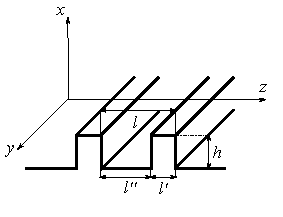
\includegraphics[width = 0.7\textwidth]{images/pdf/comb-type_structure_without.pdf}
	\caption{Гребёнка} \label{fig1}
\end{figure}
%\begin{figure}[ht]
%	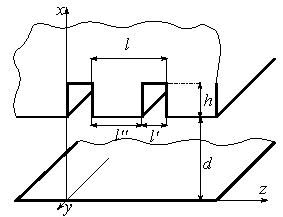
\includegraphics[width = 0.7\textwidth]{images/pdf/comb-type_structure.pdf}
%	\caption{Гребёнка над плоскостью} \label{fig2}
%\end{figure}

Часто словом <<гребёнка>>  обозначают замедляющую структуру типа <<гребёнка над плоскостью>>. Они отличаются полями. В первом случае поля экспоненциально затухают при удалении вдоль оси $x$ от структуры, во втором случае меняются по закону гиперболического синуса-косинуса \cite{Silin}.

Гребёнка над плоскостью представляет большой интерес, так как является одной из самых распространённых структур. Особенно представляют интерес поля вблизи гребней. Этому вопросу уделено внимание в статье \cite{VSTUShein3}. 

\chapter{Результаты расчётов, проведённых в семестре}

\section{Сравнение потоков с учётом магнитного поля замедляющей \mbox{структуры} и без него}

Поле $\vec{E}$ гребёнки над плоскостью в случае если поле $\vec{B}$ направлено вдоль оси $y$, поток распространяется вдоль системы, то есть оси $z$ и нет затухания, имеет вид:
\begin{equation*}
\begin{aligned}
& E_x = \sum\limits_{n=1}^{\infty} \frac{\beta_n}{\gamma_n} B_n \cosh (\gamma_n x) (\Im A_n \cos (n\omega t - \beta_n z) + \Re A_n \sin (n\omega t - \beta_n z)), \\
& E_y = 0, \\
& E_z = \sum\limits_{n=1}^{\infty} B_n \sinh (\gamma_n x) (\Re A_n \cos (n\omega t - \beta_n z) + \Im A_n \sin (n\omega t - \beta_n z)).
\end{aligned}
\end{equation*} 

Здесь:
\begin{itemize}
	%\item[] $\alpha_n$ -- коэффициент затухания $n$-й гармоники. 
	\item[] $\omega$ -- фундаментальная частота взаимодействия.
	\item[] $\beta_n = n\omega/v_n$ -- фазовая постоянная данной волны.
	\item[] $v_n$ -- фазовая скорость данной волны. По основному свойству замедляющих систем должна совпадать со скоростью потока и как следствие с переносной скоростью внешних скрещенных полей, которыми удерживается поток.
	\item[] $\gamma_n = \sqrt{\beta^2_n - n^2\omega^2/c^2}$ -- поперечное волновое число.
	\item[] $B_n$ -- амплитуда структурной функции. Её значение определяется с помощью выражения
	\[
	B_n = 2\beta_n \sqrt{\dfrac{2R_n}{\frac{\sinh 2\gamma_n d}{\gamma_n d} -2}}.
	\]
	\item[] $d$ -- ширина пространства взаимодействия (вдоль $x$). 
	\item[] $R_n$ -- сопротивление связи.
	\item[] $A_n$ --  определяется входной мощностью для данной гармоники $P_n$. 
	\begin{align*}
	& \Re A_n = \sqrt{P_n} \cos \varphi_n, \\
	& \Im A_n = \sqrt{P_n} \sin \varphi_n.
	\end{align*}
	\item[] $\varphi_n$ -- характеризует начальную фазу $n$-й волны.
\end{itemize}

Фазу будем считать равной нулю. В этом случае поле $\vec{E}$:
\begin{equation}
\begin{aligned}
& E_x = \sum\limits_{n=1}^{\infty} -\frac{\beta_n}{\gamma_n} B_n \cosh (\gamma_n x) \sqrt{P_n} \sin (n\omega t - \beta_n z), \\
& E_y = 0, \\
& E_z = \sum\limits_{n=1}^{\infty} B_n \sinh (\gamma_n x) \sqrt{P_n} \cos (n\omega t - \beta_n z).
\end{aligned} 
\end{equation}

Магнитное поле найдём из уравнения Максвелла
\(
\rot \vec{E} = -\dff{\vec{B}}{t}
\):
\begin{gather*}
- \dff{\vec{B}}{t}=
\matrixrotr{E_x}{0}{E_z}{v} =
-\left(\rotc{E_z}{x}{E_x}{z}\right) \ort{y} = \\ =
-
\sum\limits_{n=1}^{\infty} \Big( B_n \gamma_n \cosh (\gamma_n x) \sqrt{P_n} \cos (n\omega t - \beta_n z)
- \\ - 
\frac{\beta_n^2}{\gamma_n} B_n \cosh (\gamma_n x)  \sqrt{P_n} \cos (n\omega t - \beta_n z)
\Big)
\ort{y}
= \\ =
\sum\limits_{n=1}^{\infty} \frac{n^2\omega^2}{\gamma_n c^2} B_n \cosh (\gamma_n x) \sqrt{P_n} \cos (n\omega t - \beta_n z)
\ort{y}
\end{gather*}

Интегрируем по $t$ и исключаем неизменные во времени поля ("постоянные интегрирования"), получаем:
\begin{equation}
	\begin{aligned}
	& B_x = 0 \\
	& B_y = \sum\limits_{n=1}^{\infty} -\frac{n\omega}{\gamma_n c^2} B_n \cosh (\gamma_n x) \sqrt{P_n} \sin (n\omega t - \beta_n z) \\
	& B_z = 0
	\end{aligned}
\end{equation}

Магнитное поле совпадает с тем, что приведено в \cite{Silin} за исключением константы.

Все расчёты велись при параметрах: $P_n = 2$МВт, $dt = 10^{-12}$с, $B_y^{ex} = 0{,}5$Тл, $d = 1$см, площадь инжекции $2\times 2\text{мм}^2$, переносная скорость $u = 0{,}8 c$, сопротивление связи $R_n = 10$Ом. 


\begin{figure}[c]
	\parbox{0.48\textwidth}{
		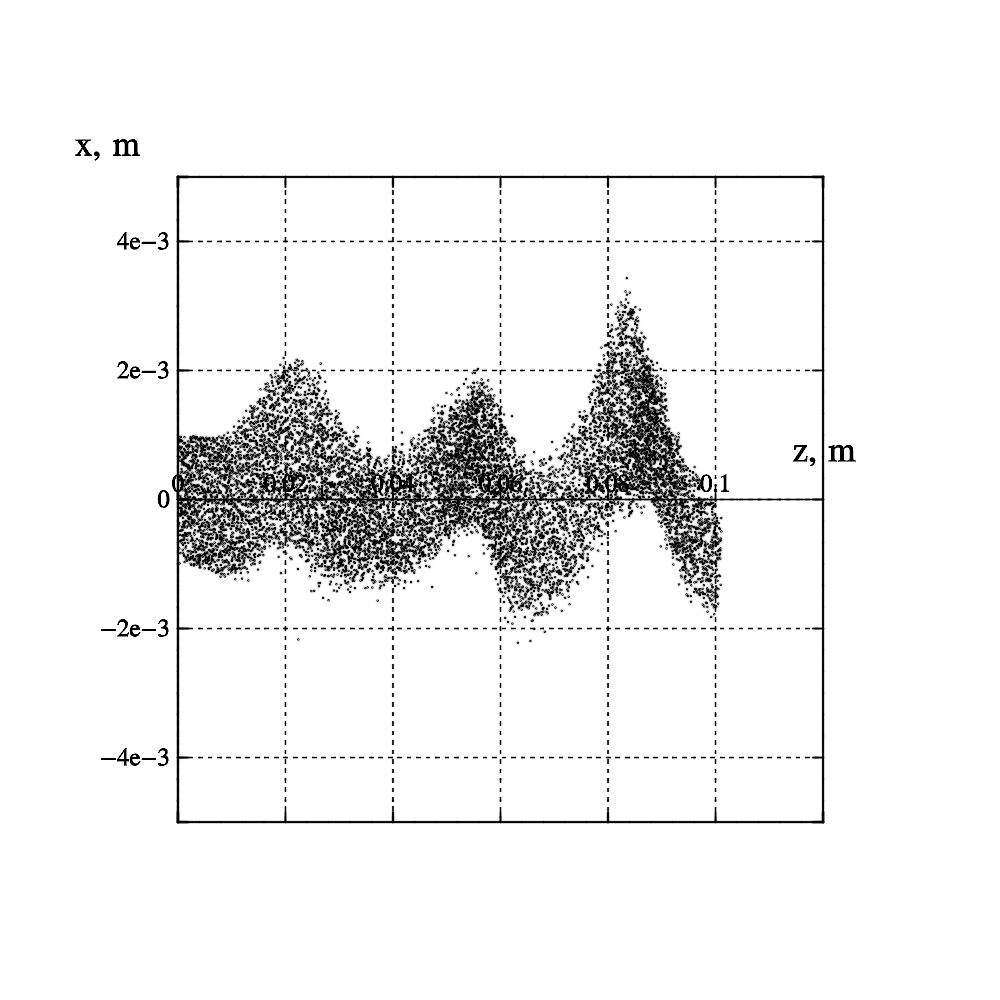
\includegraphics[width = 0.45\textwidth]{images/png/without_mf/50xz.png}
		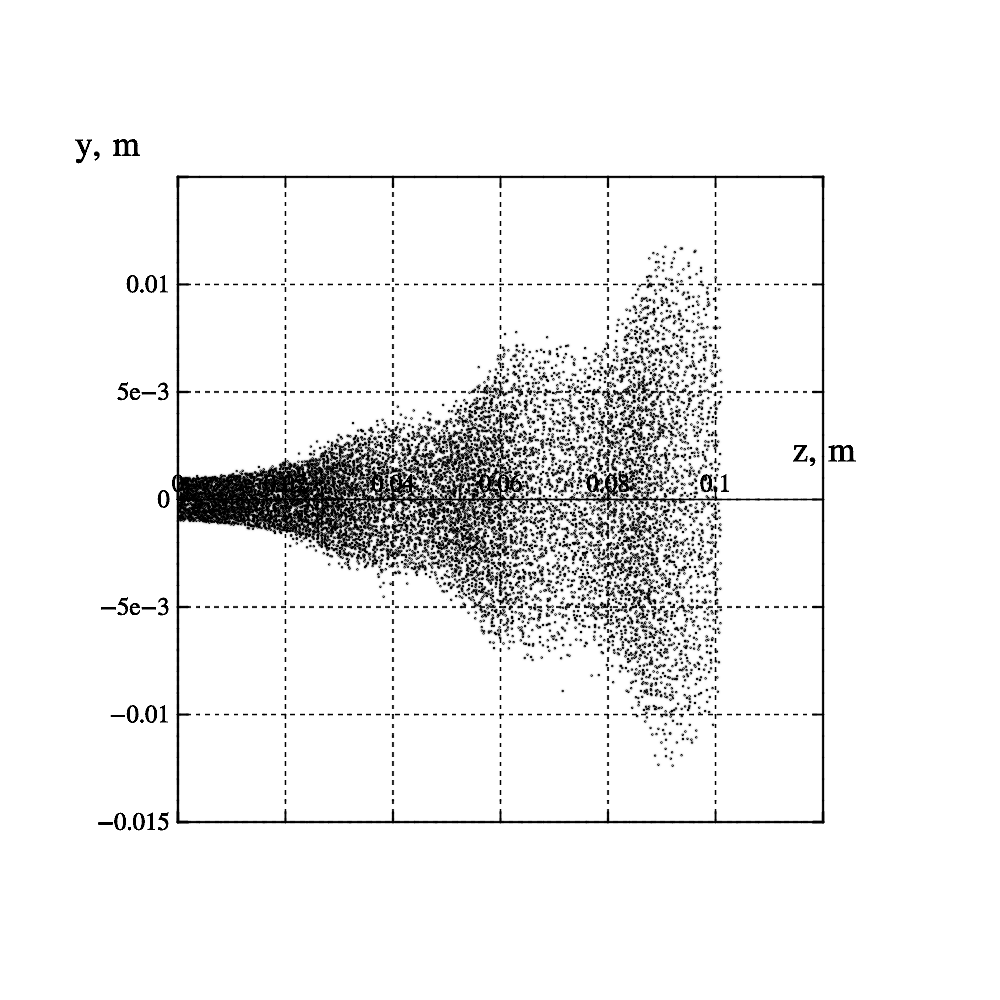
\includegraphics[width = 0.45\textwidth]{images/png/without_mf/50yz.png}
		\caption{Плоскость $xz$ и $yz$ без магнитного поля. Частота \\
			 $\omega = 50\cdot10^9$рад/c}
	}
	\quad
	\parbox{0.48\textwidth}{
		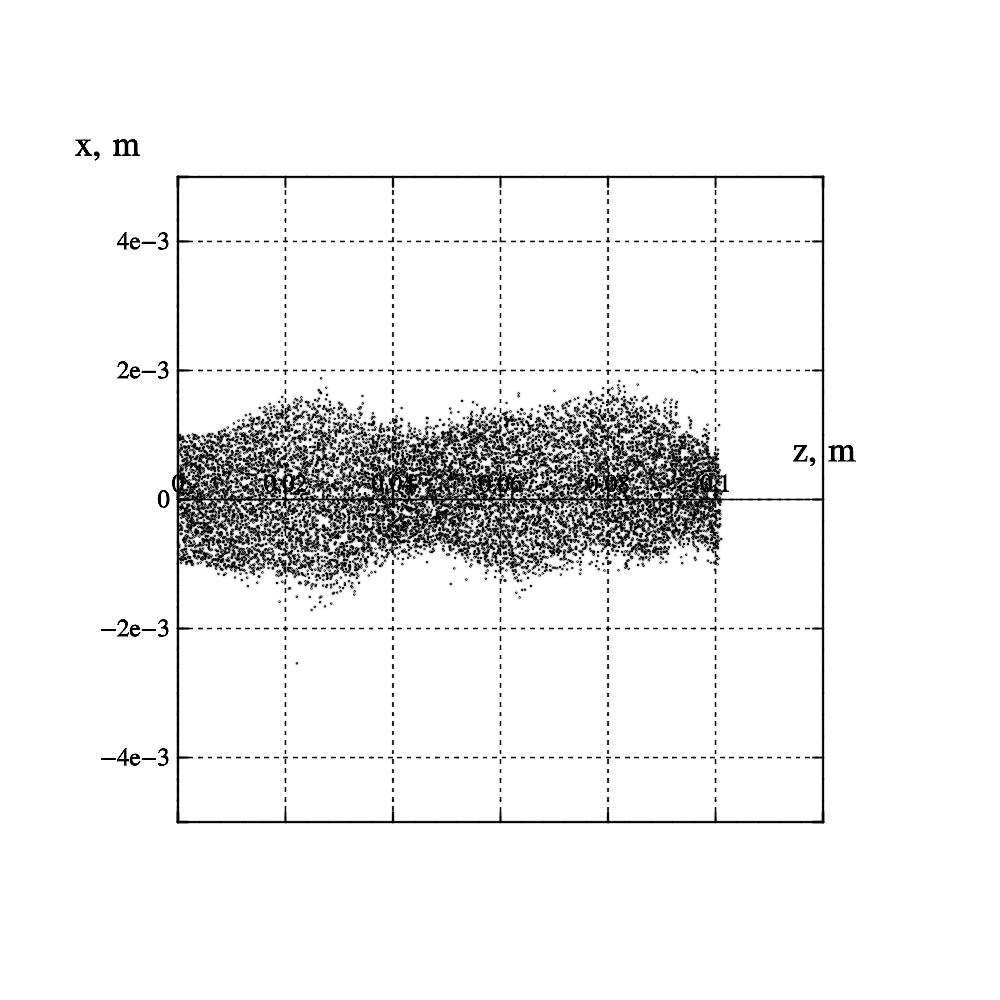
\includegraphics[width = 0.45\textwidth]{images/png/withmf/50xz.png}
		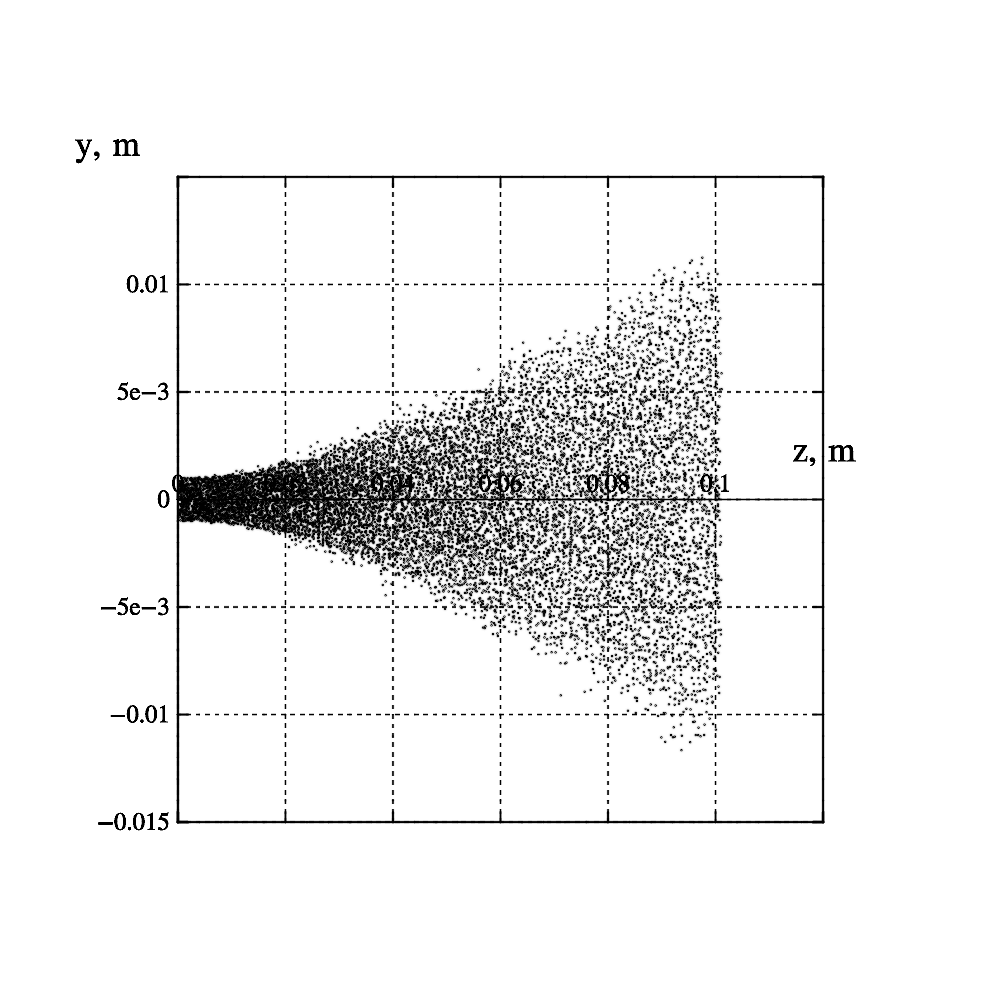
\includegraphics[width = 0.45\textwidth]{images/png/withmf/50yz.png}
		\caption{Плоскость $xz$ и $yz$ с магнитным полем. Частота \\
			$\omega = 50\cdot10^9$рад/c}
	}
\end{figure}
\clearpage
\begin{figure}[c]
	\parbox{0.48\textwidth}{
		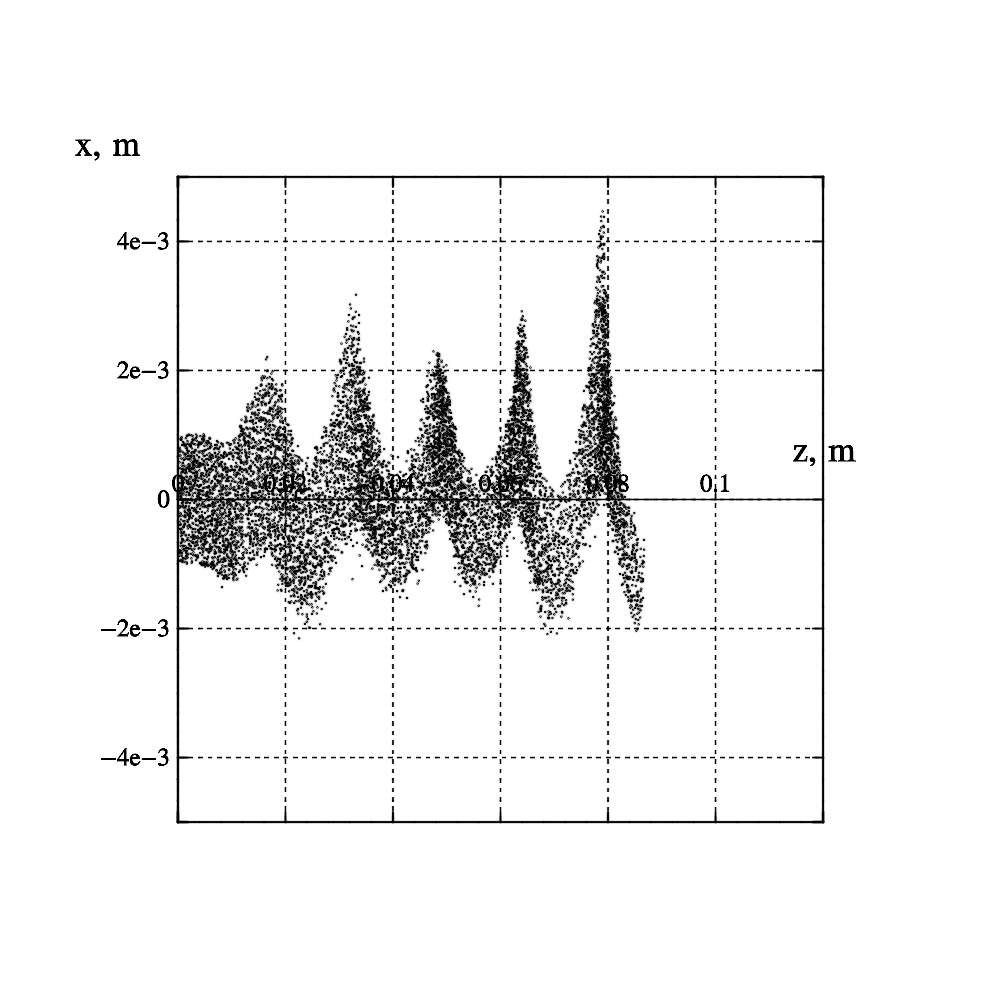
\includegraphics[width = 0.45\textwidth]{images/png/without_mf/100xz.png}
		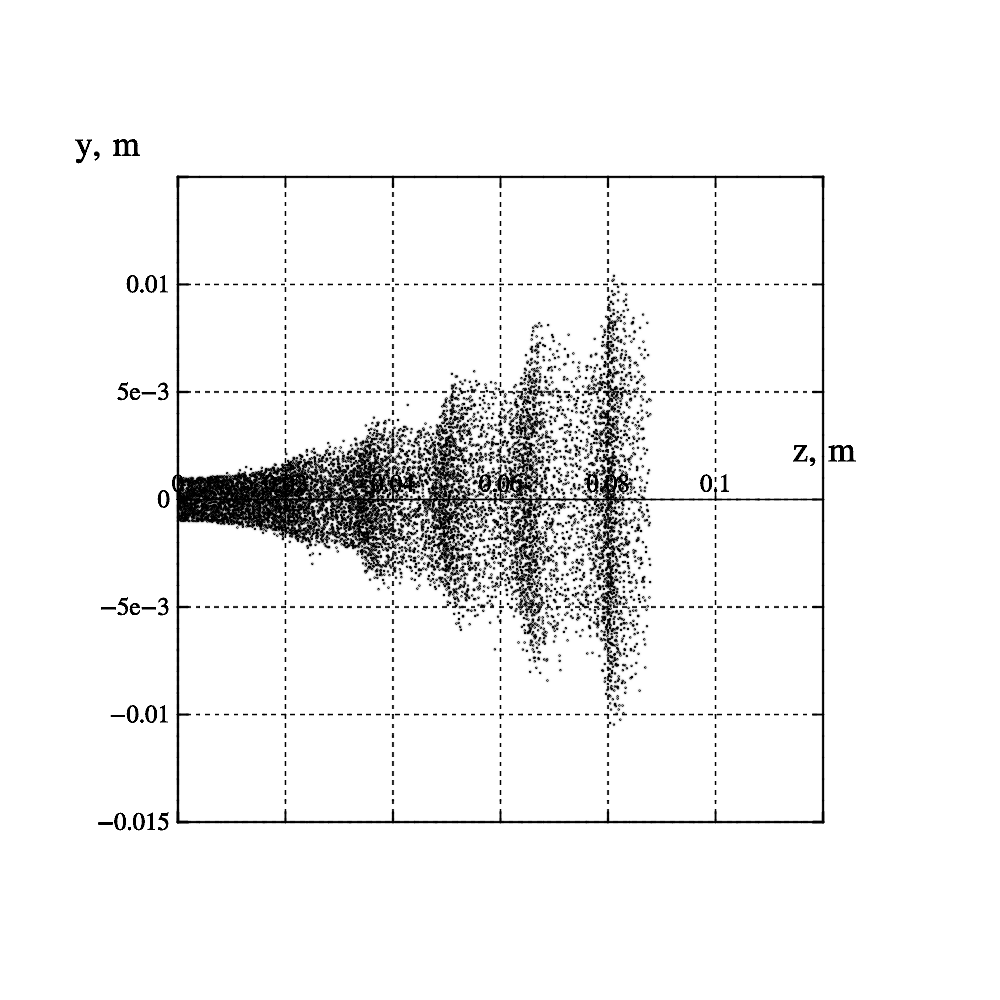
\includegraphics[width = 0.45\textwidth]{images/png/without_mf/100yz.png}
		\caption{Плоскость $xz$ и $yz$ без магнитного поля. Частота \\
			$\omega = 100\cdot10^9$рад/c}
	}
	\quad
	\parbox{0.48\textwidth}{
		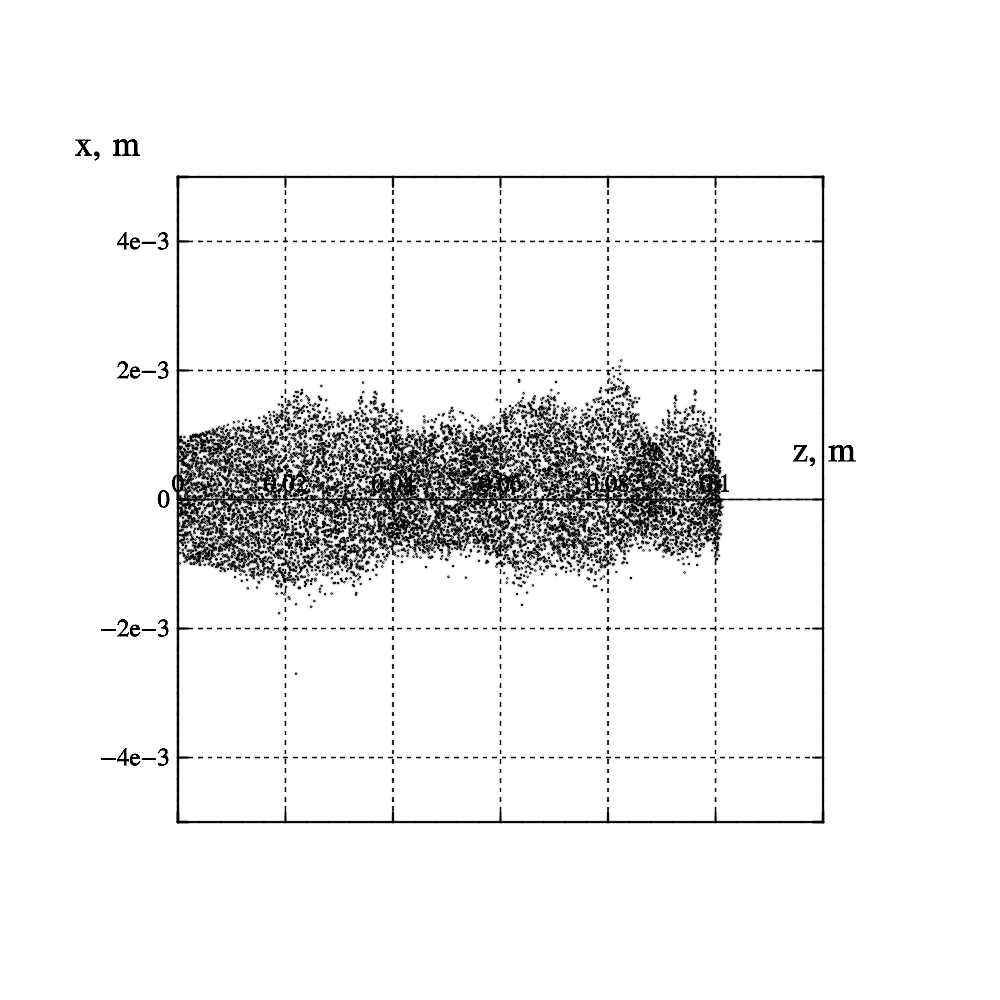
\includegraphics[width = 0.45\textwidth]{images/png/withmf/100xz.png}
		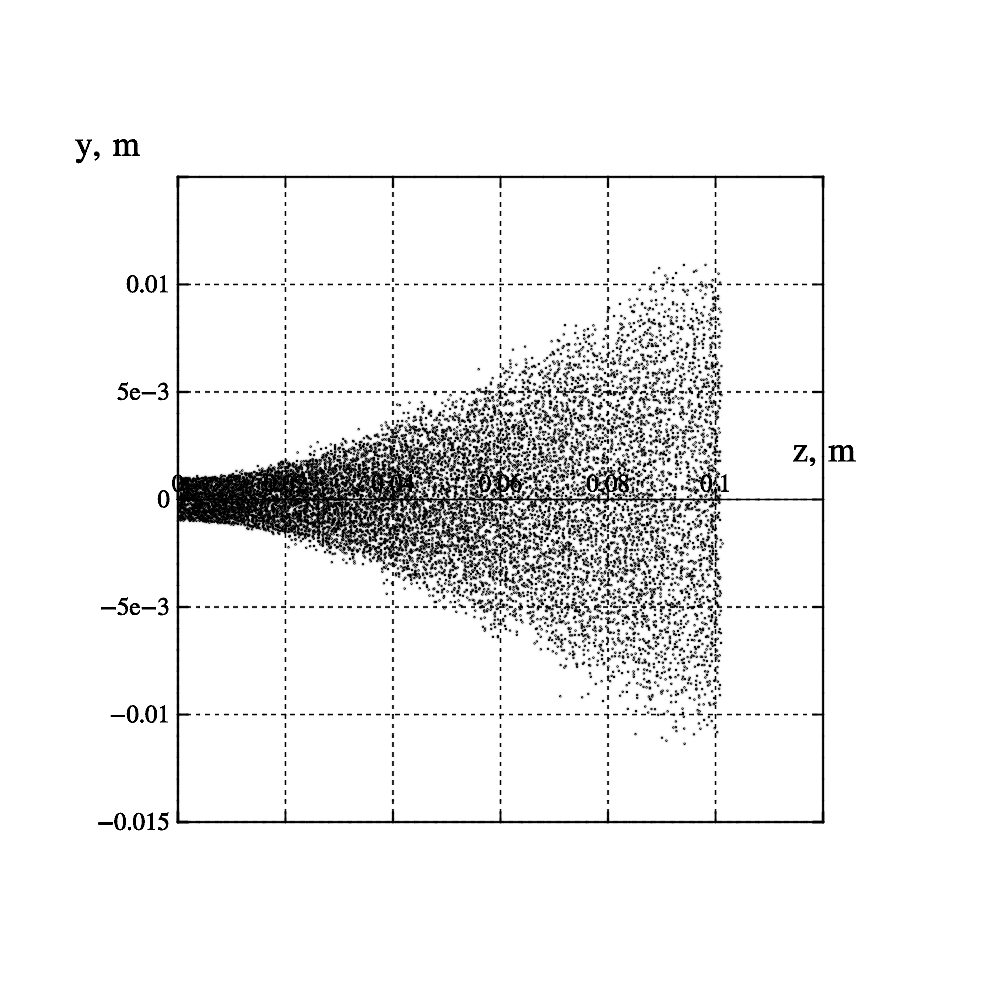
\includegraphics[width = 0.45\textwidth]{images/png/withmf/100yz.png}
		\caption{Плоскость $xz$ и $yz$ с магнитным полем. Частота \\
			$\omega = 100\cdot10^9$рад/c}
	}
\end{figure}
\clearpage
\begin{figure}[c]
	\parbox{0.48\textwidth}{
		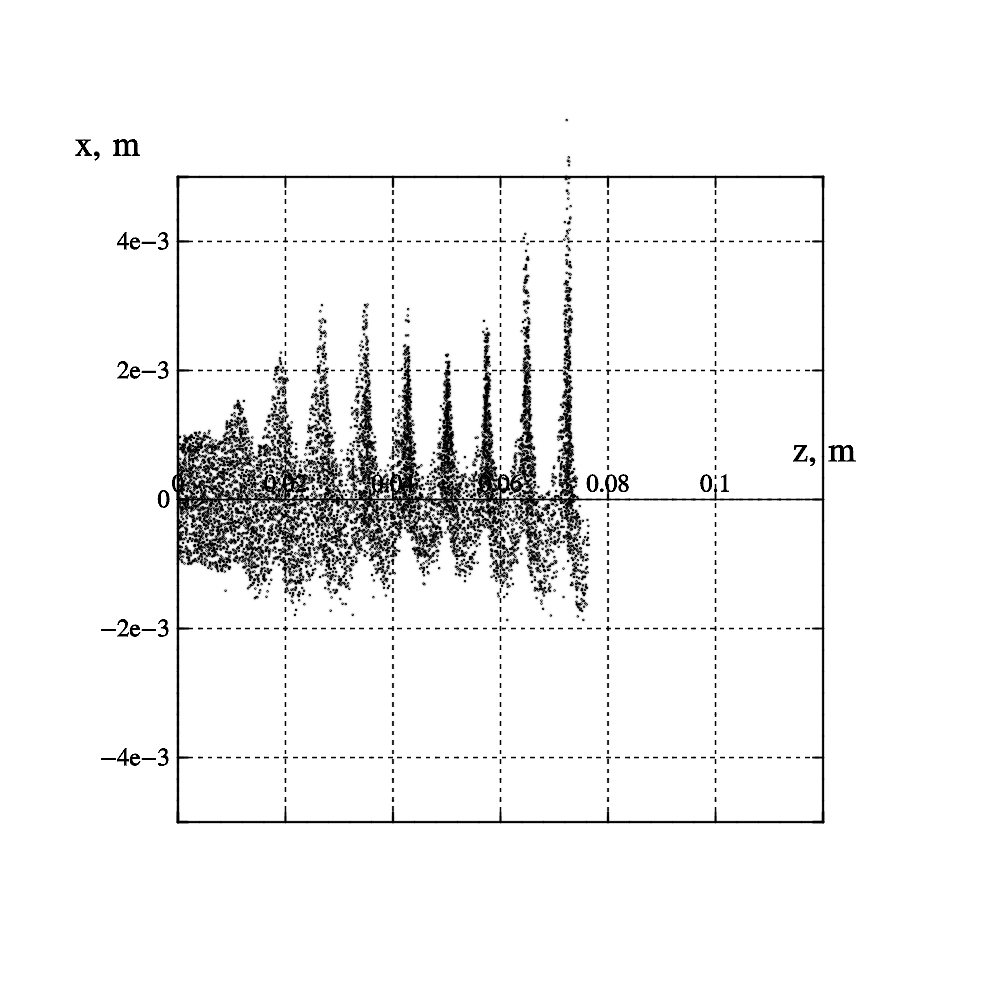
\includegraphics[width = 0.45\textwidth]{images/png/without_mf/200xz.png}
		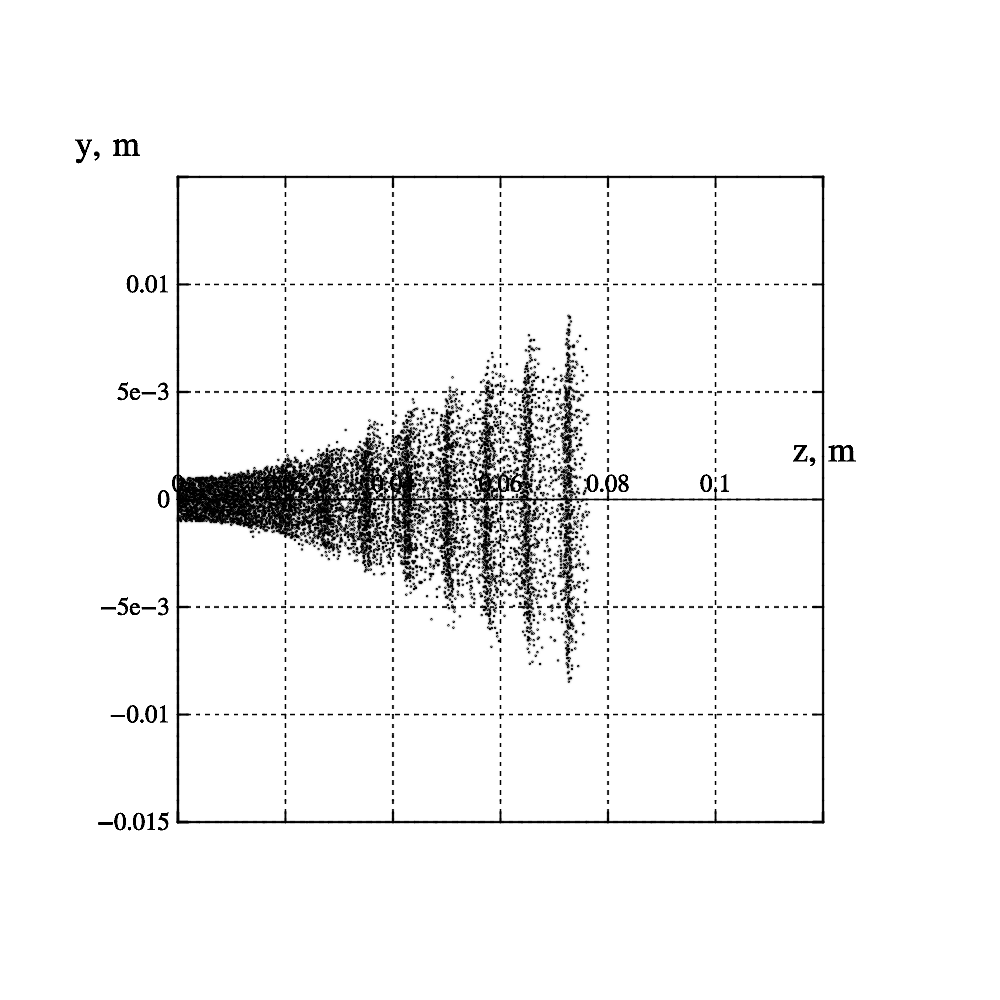
\includegraphics[width = 0.45\textwidth]{images/png/without_mf/200yz.png}
		\caption{Плоскость $xz$ и $yz$ без магнитного поля. Частота \\
			$\omega = 200\cdot10^9$рад/c}
	}
	\quad
	\parbox{0.48\textwidth}{
		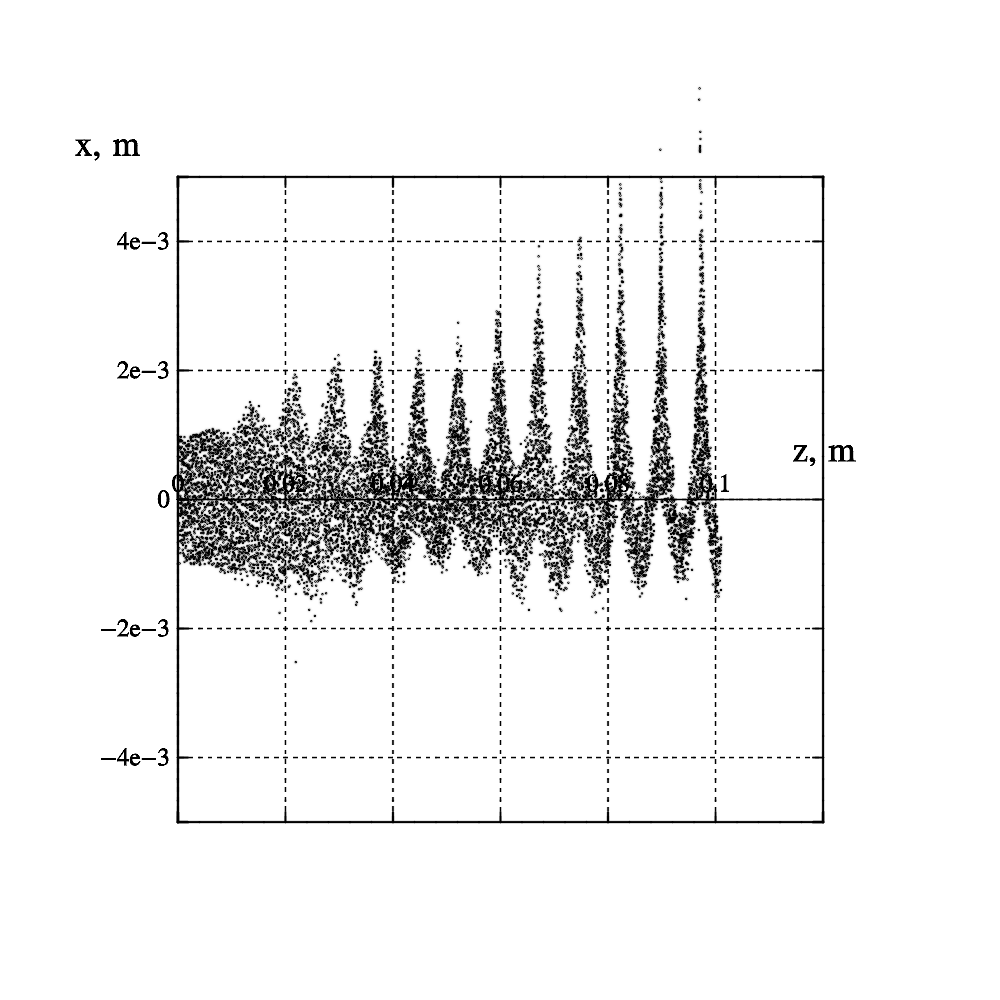
\includegraphics[width = 0.45\textwidth]{images/png/withmf/200xz.png}
		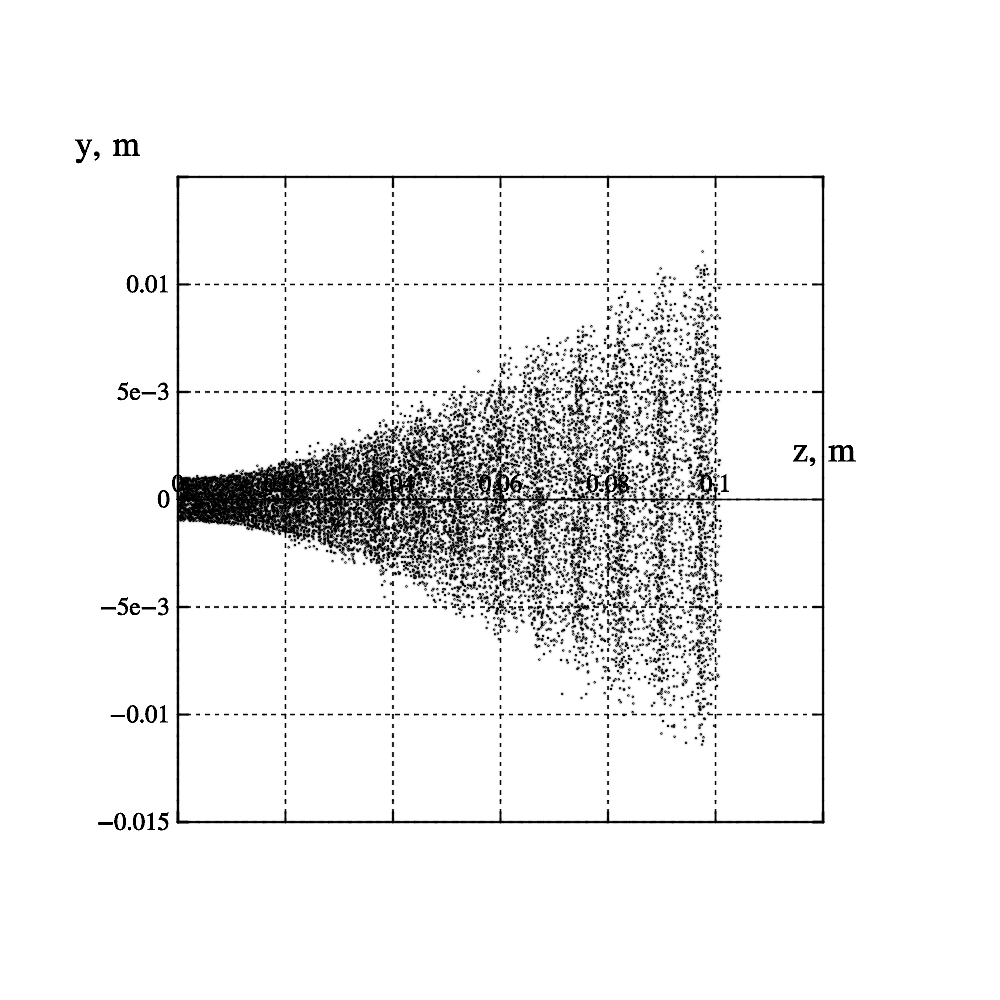
\includegraphics[width = 0.45\textwidth]{images/png/withmf/200yz.png}
		\caption{Плоскость $xz$ и $yz$ с магнитным полем. Частота \\
			$\omega = 200\cdot10^9$рад/c}
	}
\end{figure}
\clearpage

\section{Учёт дополнительных гармоник}

Предыдущие расчёты велись в случае если на поток действует одна гармоника с частотой $\omega$. Представляет интерес рассмотреть случай, в котором на поток действуют несколько гармоник структуры. При расчётах применялись параметры, приведённые выше. На рисунках \ref{fig3}-\ref{fig4} приведены формы потоков в плоскости $xz$ и $yz$. Как следует из рисунков, дополнительные гармоники вызывают осцилляции, но не приводят к оседанию электронов на катод системы.

\begin{figure}[!ht]
	\parbox{0.48\textwidth}{
		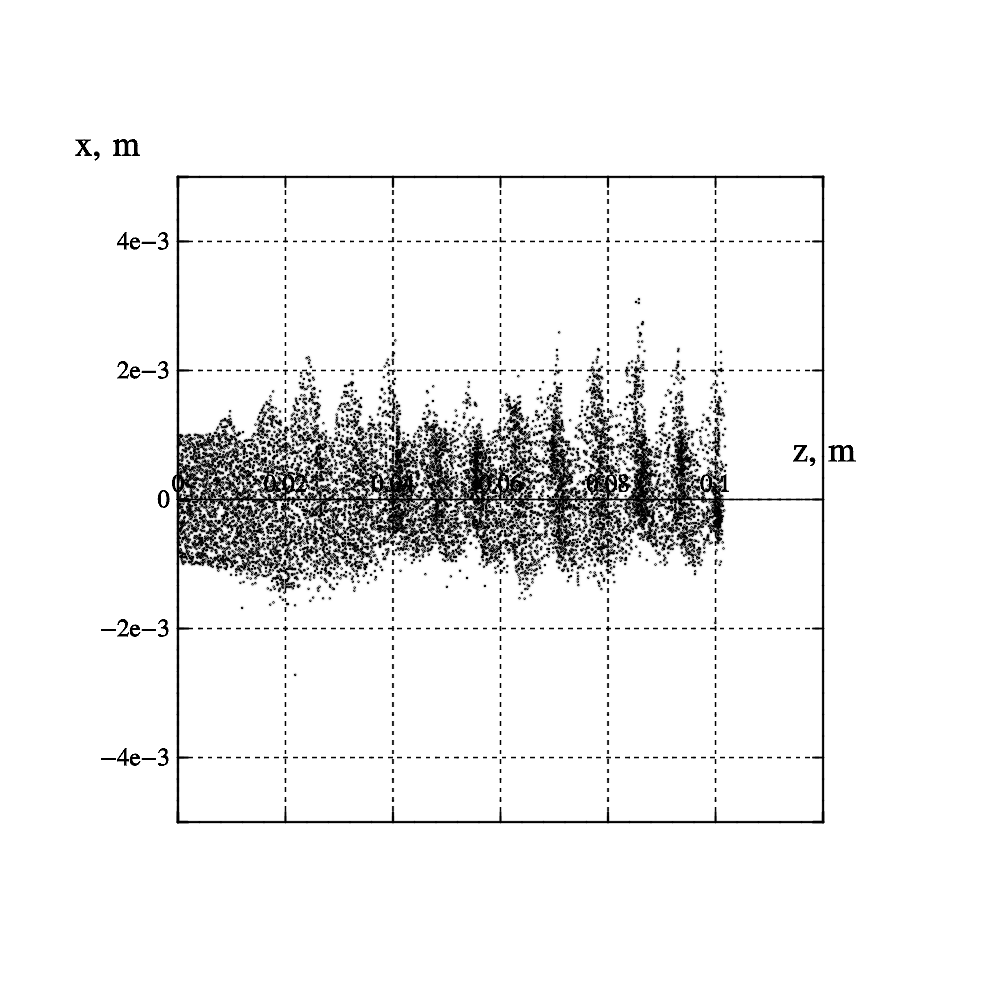
\includegraphics[width = 0.45\textwidth]{images/png/withmf/2x100xz.png}
	}
	\parbox{0.48\textwidth}{
		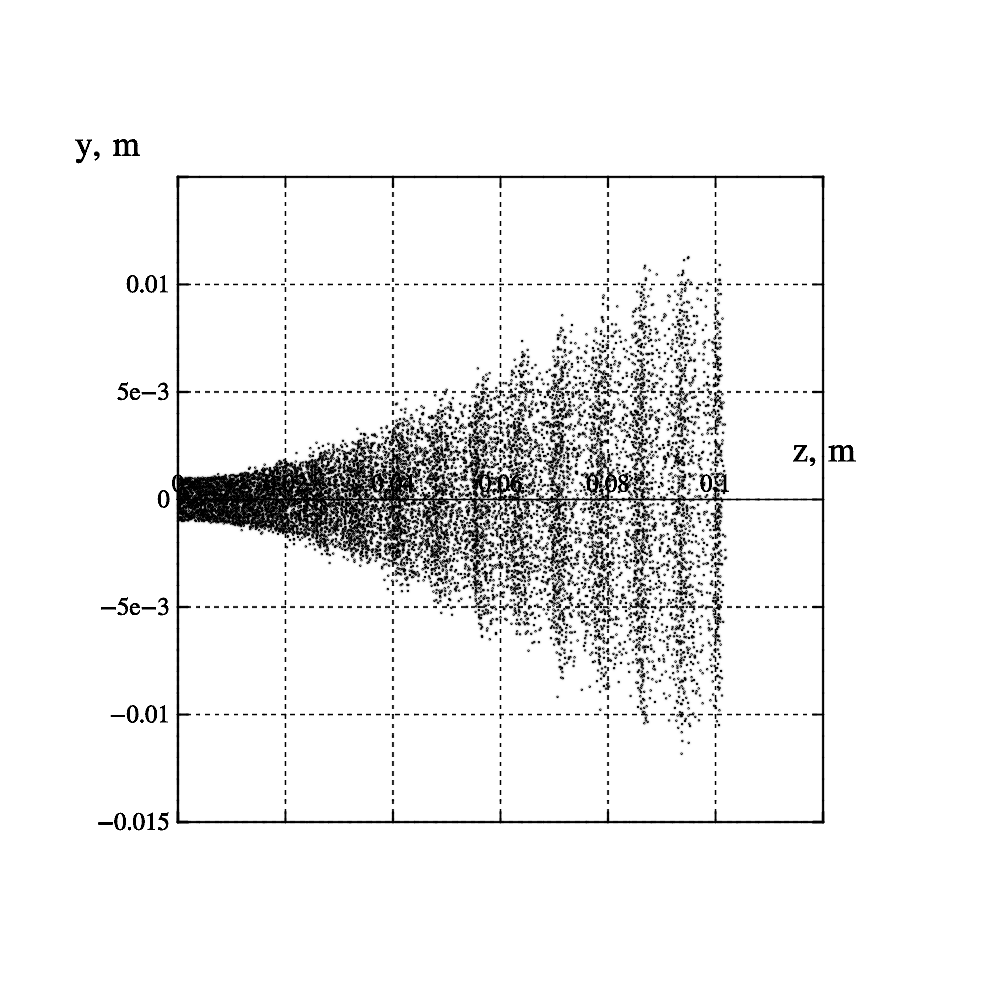
\includegraphics[width = 0.45\textwidth]{images/png/withmf/2x100yz.png}
	}
	\caption{Плоскость $xz$ и $yz$ в случае с учётом магнитного поля системы. 2 гармоники. Основная частота	$\omega = 100\cdot10^9$рад/c}
	\label{fig3}
	\parbox{0.48\textwidth}{
		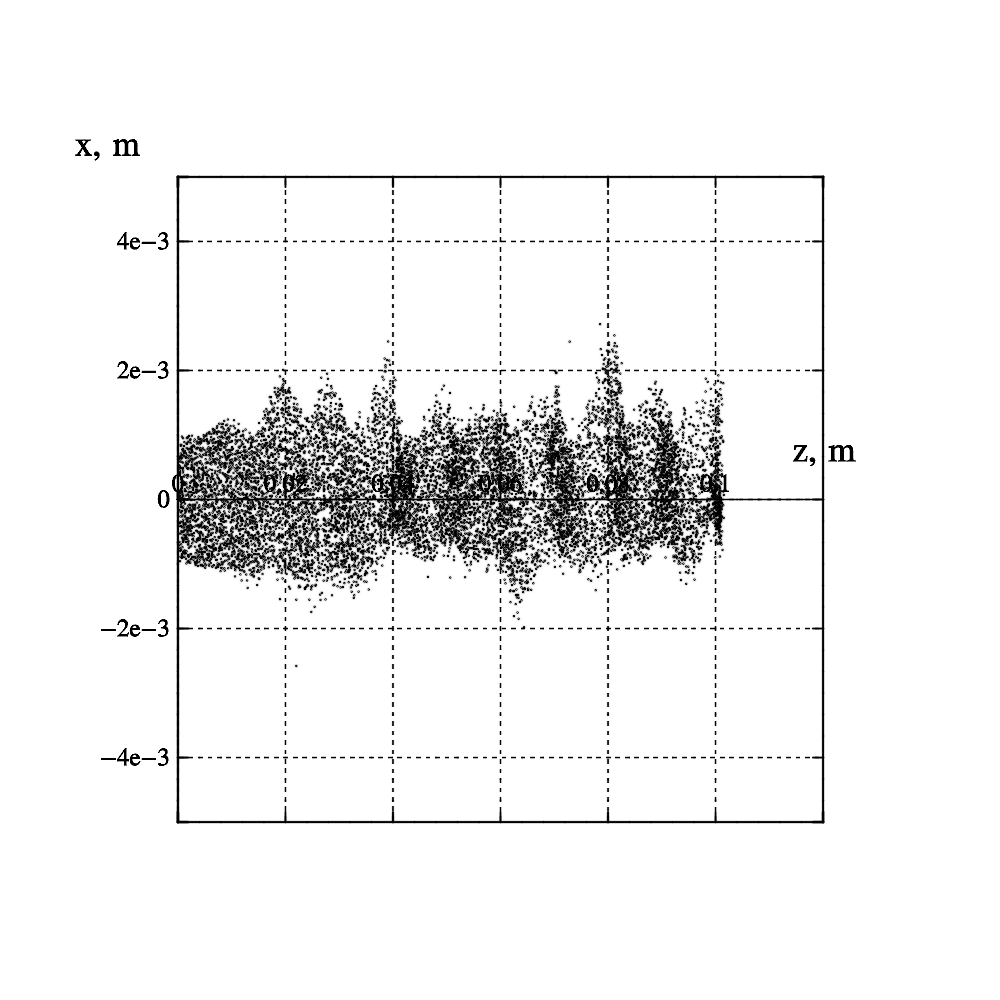
\includegraphics[width = 0.45\textwidth]{images/png/withmf/3x50xz.png}
	}
	\parbox{0.48\textwidth}{
		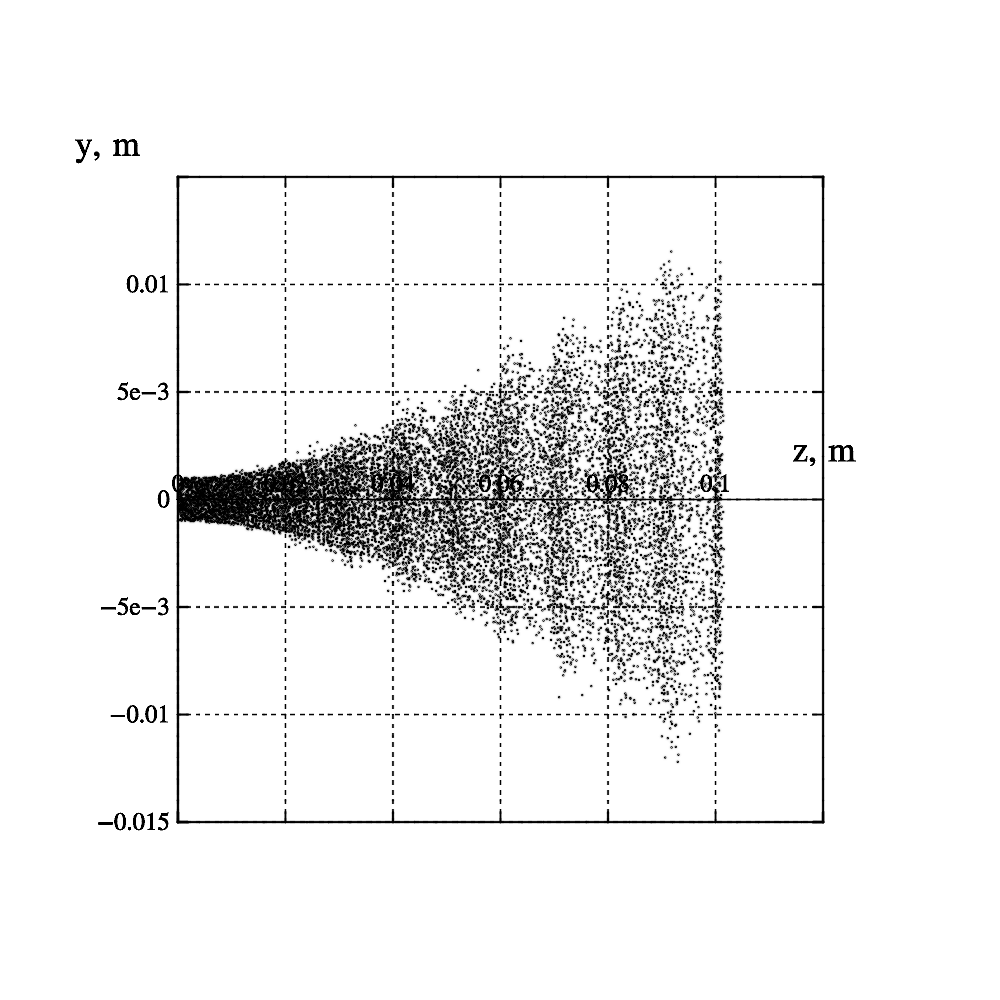
\includegraphics[width = 0.45\textwidth]{images/png/withmf/3x50yz.png}
	}
	\caption{Плоскость $xz$ и $yz$ в случае с учётом магнитного поля системы. 3 гармоники. Основная частота	$\omega = 50\cdot10^9$рад/c}
	\label{fig4}
\end{figure}


\clearpage

\addcontentsline{toc}{section}{Заключение}

\begin{center}
	\MakeUppercase{Заключение}
\end{center}

Был сделан литературный обзор и проведено моделирование электронных потоков с учётом магнитного поля замедляющей структуры, также проведены расчёты в случае если поток возбуждает не одну, а несколько гармоник. На основании результатов можно сделать вывод, что магнитное поле играет стабилизирующую роль и препятствует расширению потоков в одном из направлений, в данном случае вдоль направления $x$. С ростом частоты стабилизирующая роль магнитного поля ослабевает, электроны начинают оседать на катод структуры.

\clearpage

\addcontentsline{toc}{section}{Список использованных источников}
\bibliographystyle{gost780u}
\bibliography{lit}

\end{document}
